\documentclass[11pt, a4paper, spanish, openright, twoside]{book}
\usepackage[spanish, activeacute]{babel}
\usepackage[utf8]{inputenc}
%\usepackage[top=2.5cm, bottom=2.5cm, outer=1.75cm, inner=1.75cm, heightrounded, marginparwidth=2.5cm, marginparsep=0.3cm]{geometry}	%márgenes empequeñecidos
\usepackage[top=2.5cm, bottom=2.25cm, outer=2.75cm, inner=2.75cm, heightrounded, marginparwidth=2.5cm, marginparsep=0.3cm]{geometry}	%márgenes originalmente
\usepackage{dpg}
\usepackage{afvc}
\usepackage{pgf}
\usepackage{tikz}
\usetikzlibrary{arrows,automata,positioning}
\tikzstyle{accepting by double}= [double distance=1.6pt,double,outer sep=.5\pgflinewidth+.8pt] % esto es algo estético.
\renewcommand\shorthandsspanish{}  % para compatibilizar spanish con tikz
%Figuras
\usepackage[vflt]{floatflt}		%Entorno float-figure
%\graphicspath{/Temas/Tema01/Imagenes}

%%%%%%		chapter's style		%%%%%%%%%%%%%%%%%%%

\renewcommand{\thepage}{\arabic{page}}% Arabic page numbers\fancyhead{}
\pagestyle{fancy}
%\fancyfoot{}
%\fancyhead[RO]{}	%encabezado de pares: nombre de la sección
%\fancyfoot[LE,RO]{\thepage}	%abajo a izqda en pares, derecha en impares: numero de pagina
%\fancyhead[C]{Tecnología y Organización de Computadores} %cuadro izquierdo de pagina par: parte y contador
%\fancyfoot[CE]{Tecnología y Organización de Computadores} 
%\fancyfoot[CO]{Doble Grado Informática-Matemáticas - Universidad Complutense}
\renewcommand{\footrulewidth}{0.4pt}
%\renewcommand{\headrulewidth}{0.4pt}		% linea por debajo del encabezado
%\renewcommand{\sectionmark}[1]{\markright{{\thesection. #1}}}	

\fancyhead{}
\fancyfoot{}
\fancyhead[C]{Qué hemos hecho}	%encabezado de pares: nombre de la sección
\fancyfoot[LE,RO]{\thepage}	%abajo a izqda en pares, derecha en impares: numero de pagina
%\fancyhead[LE]{\nouppercase{\leftmark}} %cuadro izquierdo de pagina par: parte y contador
\fancyfoot[CE]{Tecnología y Organización de Computadores} 
\fancyfoot[CO]{Doble Grado Informática-Matemáticas - Universidad Complutense}


\renewcommand{\labelitemi}{$\circ$} %Primer itemize con circunferencia vacia
\renewcommand{\labelitemii}{$\cdot$} %Segundo itemize con punto pequeño
\renewcommand*{\thesection}{\arabic{section}}	% Hace que no apareca el indice de capitulos y que comience en section, GRACIAS A RUBEN
\setlength{\leftmarginii}{0em} %Segundo itemize sin sangria
\setlength{\leftmarginiii}{1em} %Tercer itemize casi sin sangria
\renewcommand{\labelitemiii}{ }
\pagenumbering{roman}
\newcommand*{\PKT}{\hbox{P}\kern-2.5pt\lower3.5pt\hbox{\small{K}}\kern-2.8pt\hbox{T}\kern-2pt}	%PiKey Team en bonito


\begin{document} 
\title{\Huge{\textsc{Jetpack -\\
	Qué hemos hecho}} \\
	\vspace{0.7cm}
	 \textsc{\Large{Tecnología y Organización de Computadores}} \\
	
\includegraphics[scale=0.3]{ucm.pdf}}
\author{{\Large{PiKey Team-}} \PKT \ : \vspace{0.2cm} \\
	Jesús Aguirre Pemán \\
	 Enrique Ballesteros Horcajo \\
	 Mayra Alexandra Castrosqui Florián\\
	 Jaime Dan Porras Rhee \\
	 Ignacio Iker Prado Rujas}
\date{\Today}
\maketitle

\newpage
\mbox{}
\thispagestyle{empty}						% Hoja en blanco, sin numeros ni nada
\newpage


\tableofcontents 							%INDICE hipervinculado

\newpage
\mbox{}
\thispagestyle{empty}						% Hoja en blanco, sin numeros ni nada
\newpage

\pagenumbering{arabic}						% Pone el contador de paginas a 1 y ahora en numeros normales

\vspace{3cm}

%ESTE FICHERO DEBERÍA SER DE UNAS 10-15 CARAS APROX.____________________________________________________

\section{Ruta de datos}
	Podemos distinguir cuatro entradas de datos diferentes:
	\begin{itemize}	
	\item Las relativas al teclado: PS2CLK es el reloj propio del teclado PS2 que funciona a  su propia frecuencia independiente 
 	del reloj de la FPGA. PS2DATA es el bus bidireccional de un bit del teclado que manda los códigos de las teclas pulsadas de manera secuencial.
	
	La gestión del teclado la realiza el módulo `control\_teclado":	Las únicas teclas reconocidas son la barra espaciadora y la tecla ``P''. El controlador del teclado detecta dichas teclas y activa las señales \texttt{pulsado} si se presiona la barra espaciadora y \texttt{pausado} si se pulsa la tecla ``P''.	
	Estas dos señales controlan el movimiento del muñeco (Barry) gestionadas por la máquina de estados del juego: Si nos encontramos en "playing" y se pulsa la ``P''  pasaremos al estado ``pausa''. Si se detecta la barra espaciadora, pasaremos
	 a ``playing'' y tanto Barry como el mapa comenzarán a moverse. El pause y el Game Over se consiguen mediante el control de los contadores de avance, que mueven el fondo, la moneda y los obstáculos, así como con el control del estado de Barry.
	Mediante estos contadores vamos accediendo a las posiciones de memoria de las ROMs que queremos en cada momento, con lo que controlamos la salida ``rgb''  que va a la pantalla, a nuestro gusto. Esta salida ``rgb'' le indica a la pantalla el color que debe dar a cada pixel
	en función de las señales \texttt{hsyncb} y \texttt{vsyncb}.

	\item El reset:	Esta señal, asíncrona, está conectada a un switch de la FPGA (en concreto el switch 1 de la placa superior correspondiente al LOC = K4) y reinicia todo el juego. Pone el nivel en el primero, por lo que se cargan tanto el fondo como los obstáculos correspondientes. Se genera un retardo para que no aparezcan de golpe. Además el contador de monedas se reinicia a cero. Se aprecia la posición del reset en la imagen.
	
	\begin{figure}[!h]
		\centering
		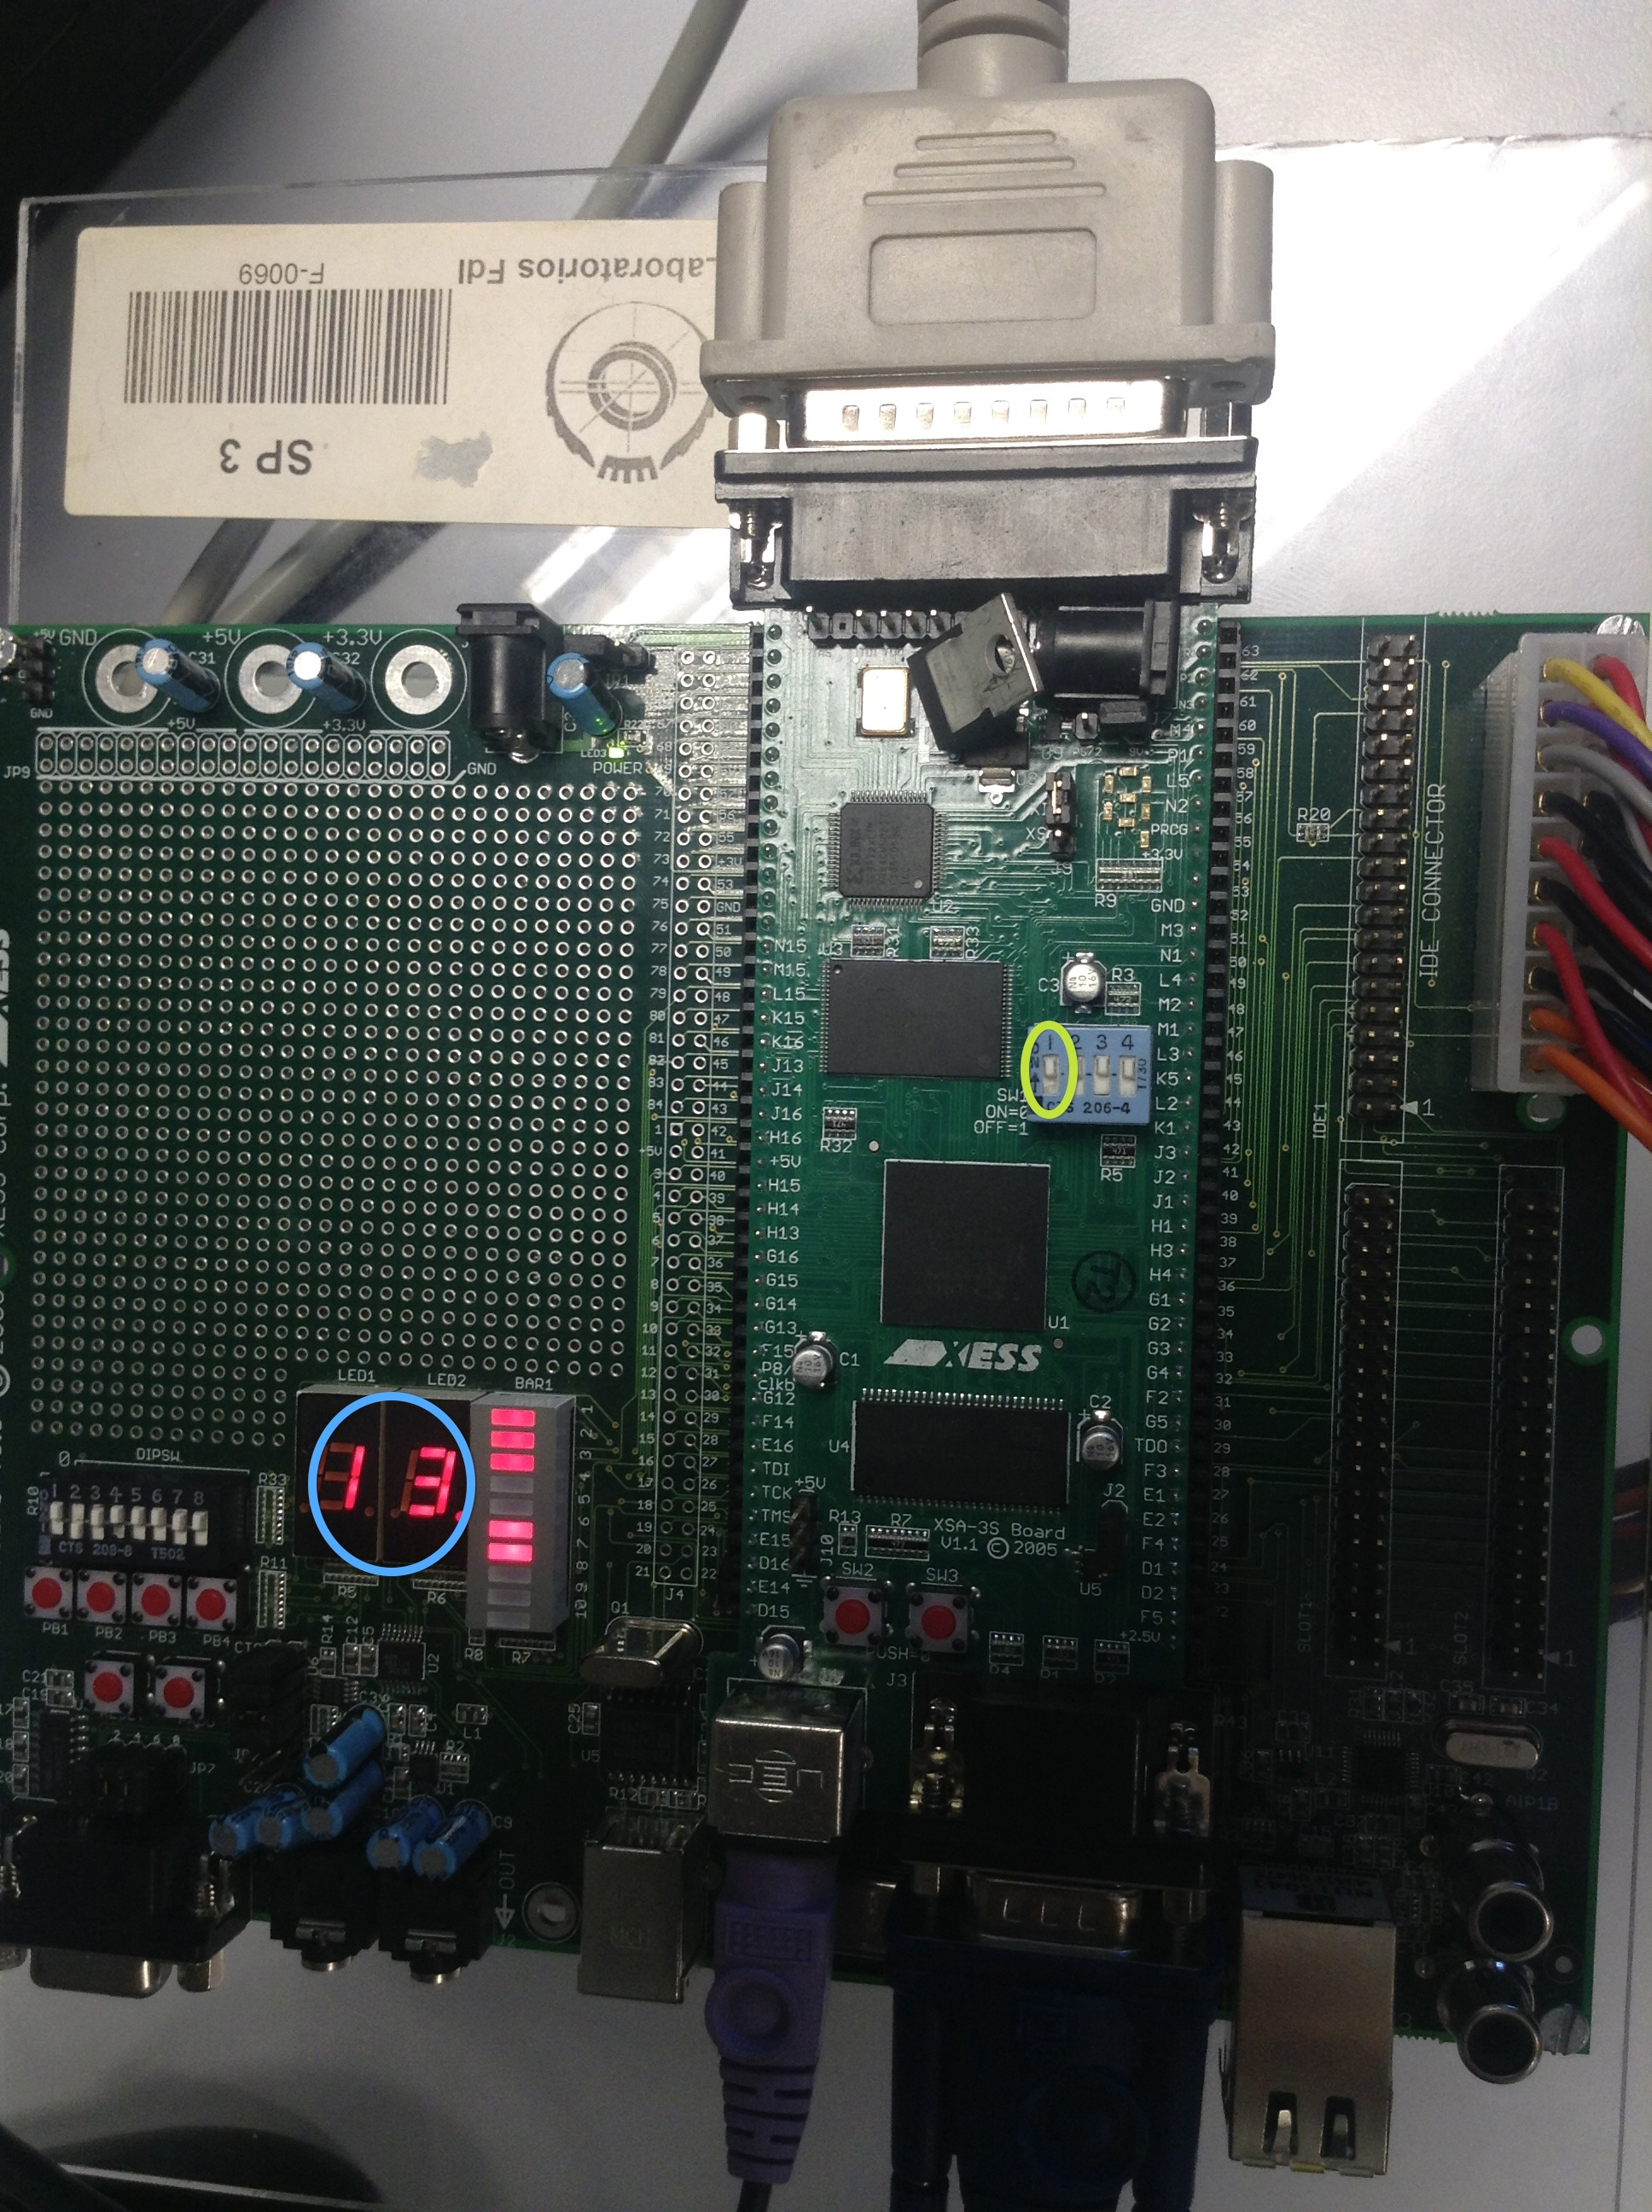
\includegraphics[scale=0.2]{fpga.jpg}
		\caption{Reset y 7 segmentos indicados en verde y azul respectivamente}
	\end{figure}
	
	\item Clock: Es el reloj de la FPGA. Está conectado a múltiples divisores que ralentizan la señal a las velocidades que se necesitan. El movimiento de los fondos, el movimiento de los obstáculos y el movimiento de Barry se gestionan mediante
	estos divisores. Además, hay uno dedicado al refresco de la pantalla que trabaja a 12,5MHz y que es el que gestiona
	
\end{itemize}
	Además podemos distinguir cinco salidas de datos:
	\begin{itemize}
	\item Las correspondientes a los siete segmentos: Las señales ``displayizq'' y ``displaydcha'' que se corresponden con los siete segmentos de la placa extendida de la FPGA. Para su gestión tenemos el módulo ``contador'' que recibe un número
	binario entre 0 y 99 y lo convierte a la salida por los siete segmentos de su representación decimal correspondiente. La entrada de este módulo la tenemos conectada a la señal ``cuenta\_monedas'', que lleva el número de monedas que ha 
	cogido el jugador.
	\item Las correspondientes a la pantalla: La señal ``rgb'' que indica el color de pixel a pintar como \texttt{hsyncb} y \texttt{vsyncb} que gestionan la posición de pantalla a pintar. La señal ``rgb'' está conectada a varias ROM y señales, y en el process ``colorear'' se gestiona qué conexión se utiliza en cada momento.
	
\end{itemize}


\section{Synthesis Report}

	Warnings:
	\begin{itemize}
	\item Señales no usadas o asignadas: Dado que el Xilinx las elimina en la optimización no le hemos dado especial importancia a estos warning.
	\item Latches: Los latches que serán borrados en la optimización tampoco les hemos tenido en cuenta. No obstante, tenemos varios latches que no hemos eliminado porque 
	facilitan el código y su eliminación exigiría un tiempo que no merece la pena.	Tenemos un latch de un bit para la señal "next\_catched". Esta señal indica si se ha cogido una moneda,
	es de vital importancia para el funcionamiento de la contabilización de las monedas, por lo que hemos optado por dejar el latch. Con más tiempo podría se eliminado haciendo un 
	estudio del valor que debe tomar en los casos para los que no está definida.	También tenemos un latch de 7 bits para la señal "next\_cuenta\_monedas". Esta señal gestiona
	 la cuenta de las monedas que lleva el jugador así como el incremento del contador cuando una nueva es capturada. Es de vital importancia, y ante la falta de un análisis detallado
	del valor que debe tomar para cada caso  hemos optado por dejar el latch. Puede observarse que los latch que tenemos pertenecen al módulo de las monedas, el último
	 que hemos implementado y para el cual no hemos podido realizar un trabajo perfecto por lo tiempos ajustados.	
	\item Width mismatch: En el código realizamos varios truncamientos de logic vectors. Como sabemos que xilinx los realiza correctamente no nos hemos preocupado de eliminar
	estos warnings, por lo que aparecen varios de este tipo.
	\item Not match array range: En la rom del game over hay una parte que no utilizamos de la imagen pero que está en memoria. Este warning se soluciona volviendo a generar una rom correcta.
	 No hemos considerado de suficiente interés corregirlo.
	\item More than 100\%: Este warning se debe a la escasa memoria que tiene la spartan3. Nuestros mapas, al no caber en memoria, son cableados y acaban usando toda la fpga. La optimización del xilinx 
	consigue reducir por debajo del 100\% este uso normalmente, pero no siempre. En la última sintetización tenemos: More than 100\% of Device resources are used. Siendo más concretos:	
	Number of Slices:  7962  out of   7680   103\%. 
\end{itemize}
	Datos de interés:
	\begin{itemize}
	\item BELS: 20748
	\item FlipFlops/Latches: 339
	\item RAM'S: 24
	\item  Number of 4 input LUTs:  14931  out of  15360    97\%  


\end{itemize}
	Clocks:
	\begin{itemize}
	\item  Minimum period: 30.328ns 
	\item 	Maximum Frequency: 32.972MHz
 	\item  Minimum input arrival time before clock: 12.179ns
   	\item Maximum output required time after clock: 22.577ns

\end{itemize}
	Memorias RAM:
	
	Number of BRAMs:    24  out of     24   100\%  

	Como ocupamos todas las RAM'S de la fpga, y ésta no son suficientes para almacenar todos los mapas, para ciertos mapas tenemos:
		The ROM description  will be implemented on LUTs because the limited number of device block RAMs.
	Esto hace que ciertos mapas se cableen, lo que ralentiza la sintetización y hace que se ocupen la mayor parte de las LUT'S de la fpga.
	Un efecto secundario de utilizar toda la fpga es que el clock skew se convierte en un grave problema, ya que debe llegar a todas 
	 las partes de la fpga.

	Otros datos de interés:
	
	Total REAL time to Xst completion: 1131.00 secs (18.85 min).

\section{Controladores}
\subsection{Introducción y estados del juego}
La función de cada señal esta explicada en \texttt{choca.vhd} y sería pesado e innecesario volver a reproducirla aquí, por lo que optamos por omitirlo.

En primer lugar, vemos que cargamos separadamente de memoria a Barry,  los mapas, los obstáculos y el cartel de ``Game Over". Por tanto, necesitaremos 5 memorias ROM diferentes. Para mostrar a Barry corriendo tenemos dos ROM, y a esto hay que sumarle las tres ROM de fondos junto a las 3 ROM de obstáculos, haciendo un total de 9 ROMs, cada una del tamaño correspondiente. 

El juego tendrá 5 estados:
\begin{itemize}
\item Game Over: Nos hemos chocado, y por tanto, la partida se ha acabado.
\item Pause: Pulsando la tecla `P'  \ paramos el juego.
\item Quieto: Barry no está subiendo ni bajando: puede estar andando o en el techo.
\item Subiendo: Al pulsar la barra espaciadora activamos los propulsores del Jetpack y Barry sube.
\item Bajando: Cuando soltamos la barra espaciadora, cortamos el combustible y Barry cae.
\end{itemize}

\subsection{Imágenes y movimientos}
%A continuación, describamos el código referente a las \textbf{imágenes y movimientos}:

Las señales $posy$ y $posx$ nos indican en qué posición estamos pintandolos obstáculos, y su concatenación, $dir\_mem$, es la dirección que utilizaremos para leer de memoria. Lo mismo ocurre con el fondo, barry, y ``Game Over".

La señal $fondo\_inter$ conecta los dos fondos que tiene el Nivel 3 (inspirado en ``Super Mario").

El process $mueve\_obstaculos$ es el encargado de refrescar la pantalla y pintar los obstáculos que salen a medida que avanzamos en el juego. Para ello borra la primera columna, desplaza el resto de columnas a la izquierda, e inserta la nueva columna a la derecha. El process $mueve\_fondo$ hace lo mismo con el fondo de la pantalla, y $mueve\_fondo\_inter$, con el fondo intermedio del Nivel 3.

	\begin{figure}[!h]
		\centering
		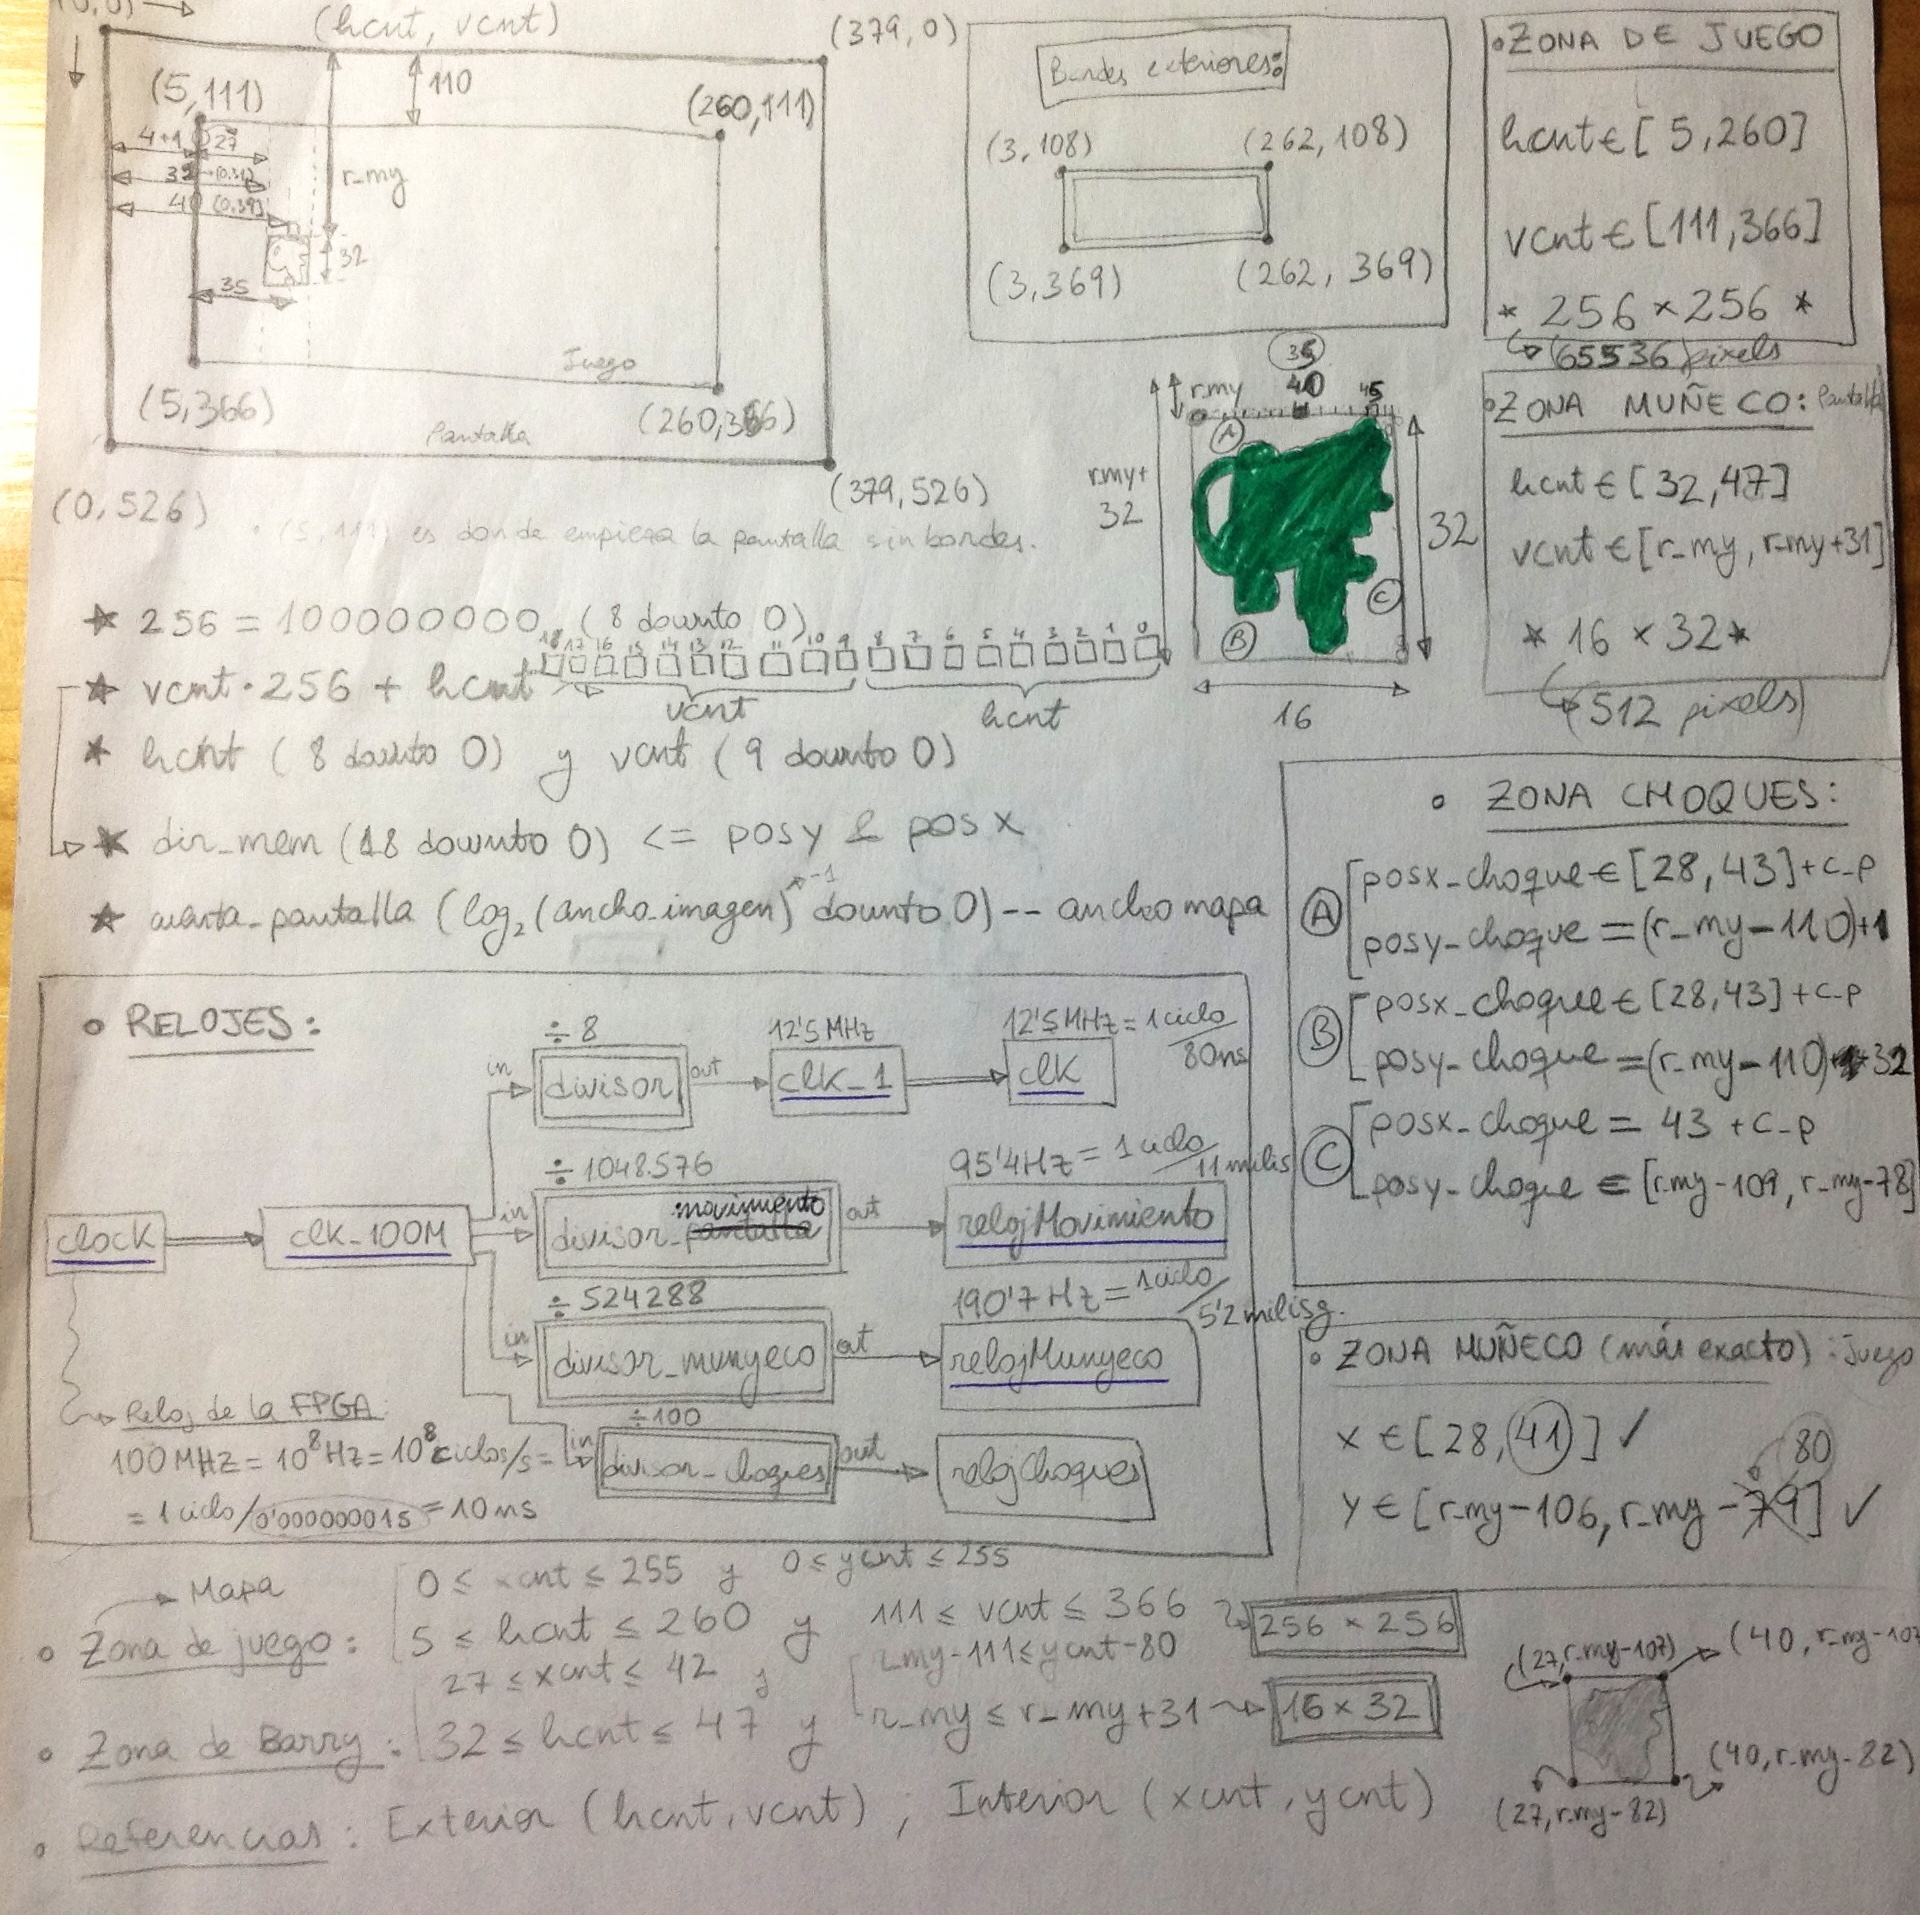
\includegraphics[scale=0.2]{calculos.jpg}
		\caption{Algunos cálculos de píxeles y algunos relojes}
	\end{figure}
	
También son importante las medidas de Barry. La imagen tiene 32x16 píxeles, se encuentra a 32 píxeles del final de la pantalla y a 27 del borde de la zona de juego. La distancia de la cabeza del muñeco hasta el final de la pantalla es de $r\_my$ píxeles, y de $r\_my-110$ hasta el borde de la zona de juego. Así, la zona de Barry es $hcnt \in [27, 40]$ y $vcnt \in [r\_my-107, r\_my -82]$.


El process $mueve\_obstaculos$ es el encargado de refrescar la pantalla y pintar los obstáculos que salen a medida que avanzamos en el juego. Para ello borra la primera columna, desplaza el resto de columnas a la izquierda, e inserta la nueva columna a la derecha. El process $mueve\_fondo$ hace lo mismo con el fondo de la pantalla.


El process $mueve\_munyeco$ se ocupa de dar la sensación de movimiento a Barry: cuando esté en el suelo, se cargarán alternativamente dos imágenes diferentes para que parezca que sus piernas se mueven.
$mov\_munyeco$ actualiza la posición de Barry en función de su estado, y $mueve\_munyeco$ actualiza el estado del muñeco en función del estado anterior y la entrada de teclado (máquina de de estados). Junto con $estado\_munyeco$ son los encargados de actualizar estado y posición de Barry.


\subsection{Niveles}
%Pasemos a analizar la parte de los \textbf{niveles}.

$clock\_estado\_nivel$ actualiza secuencialmente en cada flanco de reloj el nivel en el que nos encontramos.
El process $niveles$ se encarga del paso entre los diferentes niveles: al aguantar sin chocarnos cierta cantidad de tiempo en un nivel pasamos al siguiente, para lo que hay que cambiar obstáculos y fondo.
Hay tres estados en los niveles:
\begin{itemize}
\item \texttt{nivel 1}: en este nivel se cargan el fondo de laboratorio y los obstáculos de trampas eléctricas. Una vez se hayan conseguido $5$ ó  $5+15n<60,\ n\in\mathbb{N}$  monedas se pasará al \texttt{nivel 2}, y se activará la señal $bloquea\_obstaculo$ que evita que los obstáculos del nivel siguiente se activen de golpe, a través del \texttt{gestorCambioNivel} que hace que los obstáculos se cambien gradualmente. 
\item \texttt{nivel 2: }en este nivel se cargan el fondo de laboratorio y los obstáculos de tuberías. Al conseguir  $10+15n<60,\ n\in\mathbb{N}$ monedas se pasará al \texttt{nivel3}, activando a su vez \textit{bloquea\_obstáculos}.
\item \texttt{nivel 3: }en este nivel se cargan el fondo con nubes y montañas y los obstáculos de bolas de fuego. Al conseguir $15n<60,\ n\in\mathbb{N}$ monedas se pasará al nivel 1, y una vez se haya llegado a las 60 no se cambiará de nivel, aunque el juego continuará. 
\end{itemize}
Si quisiéramos generalizar esto para que el juego no acabara al coger 60 monedas se podría haber añadido un contador $j$ que se inicializara a 0 e incrementara cada vez que se pasa del nivel 3 al 1. De esta manera, para pasar al siguiente nivel habría que comprobar, desde el nivel 1 que los ultimos 5 bits (que representan los números del 0 al 15) de cuenta de monedas, a los que llamaremos cuenta, valgan $j\cdot 15 + 5$, desde el nivel 2 que la cuenta  valga $j\cdot 15 + 10$ y desde el nivel 3 que valga $j\cdot + 15$. 

\subsection{Choques y obstáculos}
%Pasemos a analizar los \textbf{choques y obstáculos}

El process $controla\_juego$ es el encargado de parar y reanudar el juego, así como de terminar la partida cuando nos choquemos.

En cuanto al process \emph{comprueba\_choques}, es el encargado, como su nombre indica, de ir calculando las coordenas $(i, j)$ adecuadas a comprobar si Barry ha colisionado con algún obstáculo. La idea es sencilla: en cada ciclo del reloj \emph{relojChoques} se comprueba un pixel del borde de Barry. Comenzamos en la esquina superior izquierda y vamos recorriendo los segmentos superior, derecho, inferior e izquierdo de manera continua, en el sentido de las agujas del reloj. Esto se consigue con una máguina de estados \emph{estado\_choques}, incrementando $i$ y $j$ de manera adecuada. Una vez que tenemos las coordenadas $(i, j)$ hacemos la concatenación $dir\_mem\_choque <= j\ \&\ (i + avanza\_obstaculos)$ que se conecta a las ROMs de obstáculos, obteniendo en la salida un bit que nos dice si hay o no choque, resultando en ``Game Over''. En la imagen se pueden apreciar mejor los bordes (aunque los números que ahí aparecen no son totalmente exactos).


	\begin{figure}[!h]
		\centering
		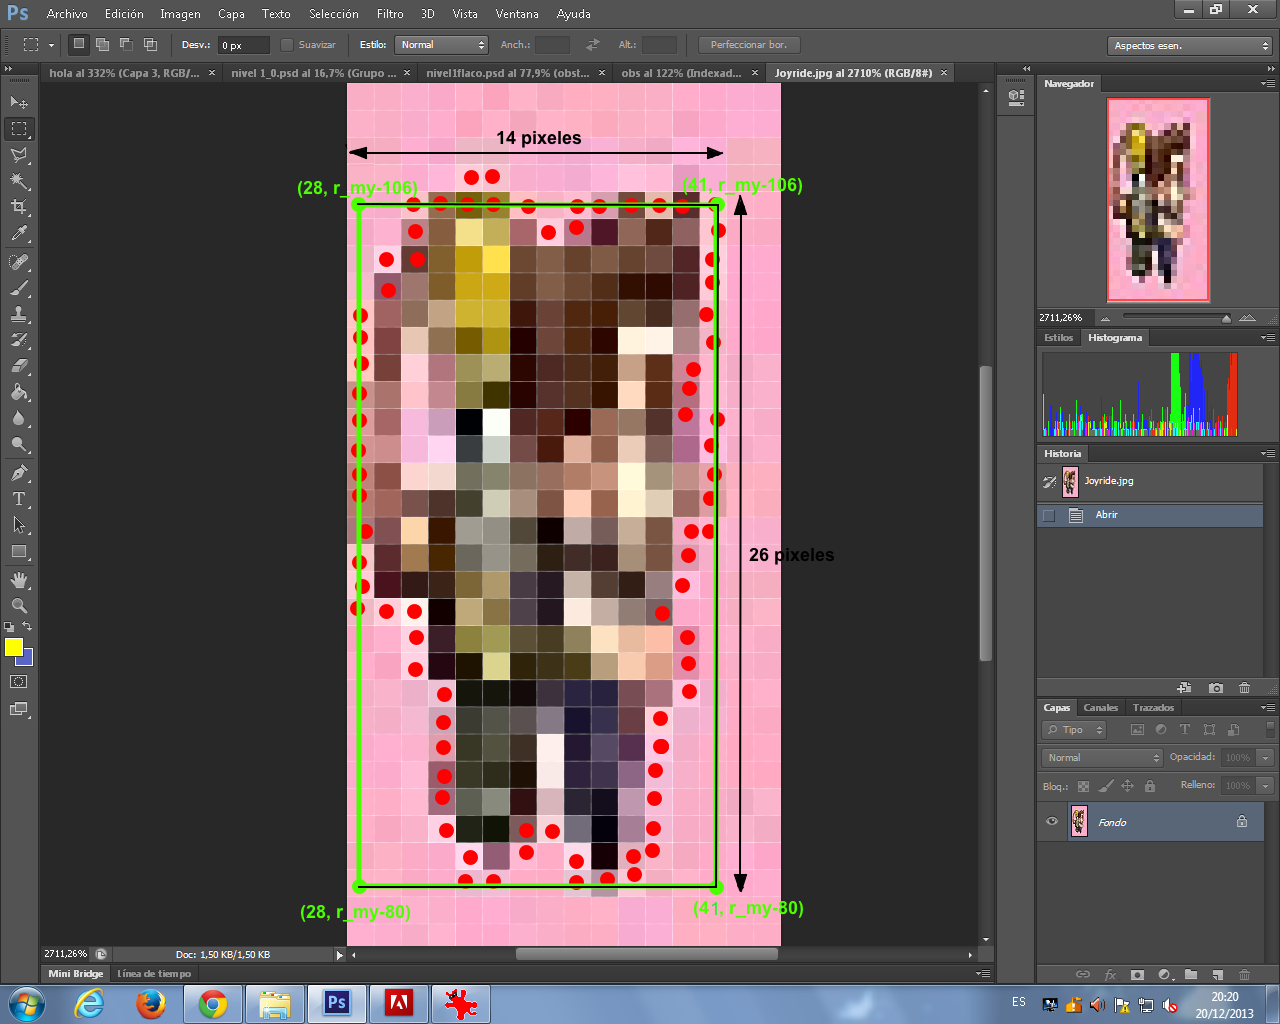
\includegraphics[scale=0.39]{barryMedidas.png}
		\caption{Algunos cálculos de píxeles y algunos relojes}
	\end{figure}

El process $pinta\_obstaculos$ lee la ROM de obstáculos y los pinta en la pantalla. En los píxeles donde no haya obstáculos se pintará el fondo del juego. $pinta\_munyeco$ hace lo mismo con la ROM de Barry, pintándolo en las posiciones de la pantalla que indica $r\_my$, la variable que almacena la posición del protagonista.

Similar es $pinta\_game\_over$, que además comprobará el estado del juego para cerciorarse de que nos hemos chocado antes de dibujar el ``Game Over".

$pinta\_bordes$ dibuja los bordes de la pantalla del juego.

Finalmente, $colorear$ decide qué pintamos en cada píxel. La pantalla se pinta pixel a pixel a una gran velocidad, para cada pixel se decide si pintar un objeto u otro según su nivel de prioridad, dejando los fondos con la menor prioridad y a Barry y los obstáculos por encima. La lista completa ordenada de los objetos que pintamos es:
\begin{itemize}
	\item Bordes
	\item Game Over
	\item Barry
	\item Obstáculos
	\item Fondo
\end{itemize}

\section{Máquinas de estados}

Principales máquinas de estados:

\begin{enumerate}

\item Niveles del juego: 

		\begin{center}
			
			\begin{tikzpicture}[->,>= stealth',shorten >=1pt, auto, node distance=4cm, thick, inner sep=4pt, bend angle=20, draw=black]
				\tikzset{every loop/.style={min distance=2mm,in=20,out=50,looseness=7}}
				\tikzstyle{every state}=[fill=blue!20,very thick, draw=blue,text=blue]

				%ESTADOS
				\node[state,initial]		(q0) []	{Nivel 1};
				\node[state]			(q1) [above right of=q0]	{Nivel 2};
				\node[state]         		(q2) [below right of=q1]	{Nivel 3};

				%TRANSICIONES
 				\path 
					(q0)	edge [bend left]			node [] 		{$5+15n<60,\ n\in\mathbb{N}$}		(q1)
				        (q1)	edge [bend left] 			node [] 		{$10+15n<60,\ n\in\mathbb{N}$}		(q2)
					(q2)	edge [bend left]			node [] 		{$15n<60,\ n\in\mathbb{N}$}		(q0)
					(q2)	edge [loop]			node [] 		{$> 60$}		();	
																
			\end{tikzpicture}
	
		\end{center}

\item Estado del juego:

\begin{center}
			
			\begin{tikzpicture}[->,>= stealth',shorten >=1pt, auto, node distance=4cm, thick, inner sep=4pt, bend angle=20, draw=black]
				\tikzset{every loop/.style={min distance=2mm,in=20,out=50,looseness=7}}
				\tikzstyle{every state}=[fill=blue!20,very thick, draw=blue,text=blue]

				%ESTADOS
				\node[state,initial]		(q0) []	{Playing};
				\node[state]			(q1) [above right of=q0]	{Game Over};
				\node[state]         		(q2) [below right of=q1]	{Pause};






				%TRANSICIONES
 				\path 
					(q0)	edge [bend left]			node [] 		{$color\_choque = 1$}		(q1)
					(q0)	edge [bend left]			node [] 		{$pausado = 1$}		(q2)
				        (q1)	edge [loop] 			node [] 		{}		()
					(q2)	edge [bend left]			node [] 		{$pulsado = 1$}		(q0);																
			\end{tikzpicture}
	
		\end{center}

\item Estados de la moneda y transiciones principales:

\begin{center}
			
			\begin{tikzpicture}[->,>= stealth',shorten >=1pt, auto, node distance=5.5cm, thick, inner sep=4pt, bend angle=20, draw=black]
				\tikzset{every loop/.style={min distance=2mm,in=20,out=50,looseness=7}}
				\tikzstyle{every state}=[fill=blue!20,very thick, draw=blue,text=blue]

				%ESTADOS
				\node[state]				(q0) []				{Invisible};
				\node[state,initial]			(q1) [below left of=q0]	{Bajando};
				\node[state]         			(q2) [below right of=q0]	{Subiendo};
				\node[state]         			(q3) [below right of=q1]	{Quieto};


				%TRANSICIONES
 				\path 
					(q2)	edge [bend right=8]			node [swap] 			{$posy\_moneda \le 115$}		(q1)
					(q1)	edge [bend right=8]			node [swap] 			{$posy\_moneda \ge 310$}		(q2)
				        (q1)	edge [bend right=5] 			node [swap] 		{$catched = 1$}				(q0)
					(q2)	edge [bend right] 			node [swap] 			{$catched = 1$}				(q0)
				        (q1)	edge [bend right] 			node [swap] 			{$estado\_juego = pause$}		(q3)
				        (q2)	edge [bend left] 			node [] 			{$estado\_juego = pause$}		(q3)
				        (q0)	edge [bend right] 			node [swap] 			{$avanza\_obstaculos = (1023)_{10}$}	(q1)
				        (q3)	edge [bend right=5] 			node [swap] 			{$playing$}		(q1);														
			\end{tikzpicture}
	
		\end{center}


\end{enumerate}
\section{Somos los mejores }
\subsection{Cronología y detalles del proceso de desarrollo}
%inicio del protecto
Tras decidir el proyecto, una de las primeras cosas que  necesitábamos era capturar las pulsaciones de teclado que hacen que Barry suba y baje, lo cual fue relativamente sencillo gracias a los ejemplos vistos en clase. Otra necesidad fue pintar imágenes en pantalla. Dibujarlas mediante process fue fácil, pero el nivel de complejidad de los dibujos era muy bajo. Tras estudiar diferentes opciones finalmente se decidió cargarlas desde ROM.
El problema ahora era generar la ROM.

%paso de imagenes a la FPGA mediante ROMs (diferenciacion entre fondos RGB y obstaculos BINario)
Para imágenes pequeñas, como podía ser el caso de la imagen de Barry, se puede escribir manualmente el valor de cada pixel de la ROM. Sin embargo, para cargar los mapas era virtualmente imposible. La solución estaba clara: mediante un programa generar la ROM automáticamente. Afortunadamente, tras investigar a fondo sobre las memorias ROM y su uso en códigos VHDL, conseguimos encontrar un programa, hecho por la Universidad Rey Juan Carlos, que convertía las imágenes en PPM a ROM. Paso seguido comenzamos a diseñar los niveles que posteriormente se pasarían a ROM con la ayuda de dicho programa. Para tal efecto se usó el programa Adobe Photoshop, creando mapas adaptados 

 %creando fondos y obstaculos (.BMP)
Se crearon dos fondos, el laboratorio y el de nubes y árboles. Se comprobó que cargando fondos muy grandes y con gran cantidad de colores la rom que se generaba era demasiado pesada para Xilinx y la FPGA, y el proyecto nunca terminaba de sintetizar. Además nos dio un aviso de que la ROM no estaba siendo implementada como ROM, sino usando muchos componentes distintos. Debido al gran tamaño de la imagen (1024 pixels de ancho) y al elevado número de colores (256) decidimos reducir ambos aspectos, siendo el nuevo ancho de 256 pixels, y 3 el número máximo de colores. Aunque creamos imágenes de fondos con solo 3 colores, la imagen sufría una compresión y descompresión durante el proceso que seguíamos para obtener la ROM, haciendo así que incrementara de manera muy notable el número de colores usados. Esto provocaba de nuevo que no se terminara de sintetizar el proyecto. Para detectar que el fallo al nuevo número de colores, tuvimos que crear un programa en \texttt{C++} que contara el número de colores. De esta manera se rehizo el proceso, evitando que la imagen se comprimiera y descomprimiera. Aún así, al ir aumentando el número de fondos y obstáculos para cubrir cada nivel, el tiempo de sintetización e implementación aumentaba de manera preocupante, por lo que se decidió crear solo tres fondos y tres obstáculos. En el caso del fonde de nubes y árboles, al ser dos fondos en uno, cada uno con su propia ROM, se consiguió mostrar el doble de colores. Además la imagen guardada en cada ROM es solo un fragmento pequeño del fondo que se ve en pantalla, el efecto se consiguió repitiendo la imagen.
La razón de usar dos fondos en uno en el nivel 3 fue que así, poniendo un reloj distinto a cada fondo, se conseguía una sensación de profundidad espacial. Este efecto de profundidad también se consiguió con los obstáculos, poniéndoles un reloj más rápido que el del fondo. 

Para los obstáculos, que tenían que ser tres, decidimos que solo tuvieran dos colores, es decir, que fueran imágenes binarias, lo que conllevó a que la ROM nos indicara donde había obstáculo y donde no. Gracias a esto último los obstáculos se pintan del color que se indica en el programa principal y no en la ROM.

La imagen de Barry y el primer fondo se inspiraron fielmente en los originales de \emph{Halfbrick Studios}. El resto de fondos y todos los obstáculos fueron dibujados a mano por el equipo. La imágenes debían ser todas mapa de bits BMP para poder restringir bien los colores y luego se transformaban a PPM para seguir el proceso de transformado y llegar al programa.


%%%%%%%%%%%%%images, if u want%%%%%%%%%%%%%



%movimiento de fondo y obstaculos
Una vez solventado la carga de imágenes a nuestra aplicación, había que darle movimiento a los mapas, lo cual avanzó enormemente el apartado visual del proyecto.


%transicion entre niveles

%choques
No obstante, este juego no tendría sentido sin obstáculos de por medio con los que chocarse.
Este fue uno de los grandes escollos del proyecto: detectar el choque.
Finalmente, decidimos pintar los obstáculos de un color determinado para comprobar si Barry ocupaba el mismo píxel que el obstáculo y dar por finalizada la partida.

Una vez decidida la estrategia llegaba el momento de implementarla, cosa que fue bastante más complicada de lo esperado, y que finalmente Iker resolvió elegantemente con una comprobación constante circular del perímetro exterior de la imagen de Barry.

Al crear nuevos niveles vimos que sería mejor añadir nuevos colores a los obstaculos para añadir más variedad, por eso decidimos modificar la ROM para que solo almacenara un bit en cada posición, significando que si el bit está a uno hay obstáculo y si está a 0 no lo hay. De esta manera se podía elegir el color de cada obstáculo en el nivel correspondiente y en vez de comprobar el color para ver el choque solo hacía falta comprobar si el bit estaba a uno o no. 


%monedas (pantalla y contados)
Ahora teníamos choques y movimiento de los mapas, y faltaba darle un objetivo al juego: conseguir el máximo número posible de monedas. Para ello teníamos que pintarlas, chocarnos con ellas, y borrarlas de la pantalla tras el choque, además de mostrar por el display 7 segmentos el número de monedas acumuladas.

Detectar el choque ya sabíamos cómo, pero eliminar la moneda y aumentar el contador se tornó más difícil de lo que parecía, puesto que había que realizar una gran distinción de casos según el estado de la moneda (subiendo, bajando, quieta, invisible...). Además, una vez chocara con Barry había que borrarla de la pantalla hasta que volviera a aparecer metros más adelante en el mapa. El hecho de que la moneda se moviera y no estuviese quieta en el mapa complicó la implementación pero dotó al juego de un aspecto visual mucho más desarrollado.











Hemos conseguido reproducir fidedignamente el videojuego $Jetpack Joyride$, incluyendo varios niveles diferentes, posibilidad de recoger monedas (y contar cuántas hemos recogido)...

\subsection{Orgullosos de algo en particular...}

Orgullosos de utilizar fondos reales creados por la mejor diseñadora gráfica del doble grado. Orgullosos de jugar con un muñeco real en vez de mover un pixel. Orgullosos de unos choques tan
 currados que permitirían generalizar las colisiones a tres dimensiones, pues son independientes del buffer de pantalla. 

Orgullosos de la habilidad del mejor 'finder' del doble grado para buscar en la web programas útiles. Y orgullosos de que Barry corra cuando está en el suelo.

\subsection{Por qué ha sido bueno ser 5...}
Formar un equipo de 5 personas ha sido clave para el éxito de nuestro proyecto, puesto que nos ha permitido trabajar en paralelo en un mínimo de 3 tareas simultáneas. Nos ha 
permitido crear una aplicación de gran envergadura que no habría sido manejable para un equipo más pequeño.
Además, aporta muchos puntos de vista diferentes para resolver un problema que surja durante el desarrollo del juego.




\subsection{Dificultades añadidas por ser 5...}

Al ser 5 personas, en todo momento había dos grupos trabajando simultáneamente sobre la aplicación, lo que obligaba a hacer un merge todos los días tras este trabajo. Este desarrollo en paralelo
creaba en ocasiones bastantes dificultades, ya que podía ocurrir que en distintas líneas de desarrollo del trabajo se tocara la misma parte del código,  lo cual creaba complicaciones a la hora de juntar el trabajo. Además, 
obligaba a crear unos buenos comentarios para que cada grupo entendiese el trabajo del otro. 

Otra dificultad añadida es la de coincidir los 5  en el laboratorio para trabajar conjuntamente con las fpgas.

\section{Qué y por qué no funciona}
Funciona todo porque somos los mejores (ver apartado 3). Sin embargo, otros añadidos si hubiésemos dispuesto de más tiempo podrían ser:
	
\begin{itemize}
	\item Menú principal.
	\item Posibilidad de elegir personaje. Se barajaron varias opciones pero no fue posible incluirlo.
	\item Posibilidad de elegir personaje.
	\item Vehículos utilizables al almacenar un número determinado de monedas. En este caso, los mapas cambiarían pasado un tiempo en lugar de cada 5 monedas recogidas.
	\item Mejorar la  manejabilidad del personaje para que acelerase al subir y flotase al comienzo de la bajada. 
	Este apartado se intentó implementar pero fue descartado puesto que el tiempo que requería no era consonante con la mejora del juego con su añadido.
	Este añadido  para mejorar la experiencia del usuario, podría no ser tal viendo el éxito del FlappyBird, que incluye una manejabilidad similar a la de nuestro juego.
	\item Contador de número de metros recorridos. Este apartado también fue considerado y comenzado, pero requería un tiempo del que no disponíamos.
	\item Generador aleatorio de obstáculos, utilizando el de las monedas con ciertas modificaciones en la práctica.
	\item Contador de monedas y contador de metros recorridos en pantalla.
	\item Creación de un juego paralelo independiente que solo consiste en coger monedas que aparecen aleatoriamente. Dada nuestra experiencia jugando, creemos que este minijuego podría llegar a arrasar a nivel mundial.
		\item Mejora de la exactitud de los choques.
		Nótese que la forma en que están implementados los 
		choques se aproxima la figura de Barry como un rectángulo.
		Esto podría mejorarse con una aproximación con más segmentos a su figura, pero llevaría muchos más cálculos e implementación que no añaden demasiado. Ésta inexactitud se nota sobre todo al chocar 
		con la parte de atrás de los pies del muñeco.
\end{itemize}


\section{Bibliografía}
Reutilización de código:

Ha sido de gran utilidad el software de la Universidad Carlos III que permite pasar una imagen en formato PPM (Portable Pixel Map) a ROM. Esto ha posibilitado la carga de mapas muy realistas y que aprovechan al máximo la capacidad de la FPGA.
Precisamente este fue uno de los principales problemas que encontramos al inicio de nuestro proyecto, y esta herramienta permitió solucionarlo de manera elegante y funcional. 

El proceso para convertir una imagen cualquiera a una ROM es el siguiente:
\begin{enumerate}
\item Convertimos la imagen a formato PPM mediante un programa de edición de imágenes (por ejemplo IrfanView).
\item Desde línea de comandos, ejecutamos la aplicacion $ppm2rom$ seguida de los parámetros 9(bits por cada pixel) y 1 (número de memorias ROM).
\item Conectamos la ROM al módulo principal del proyecto, y ya podemos mostrar la imagen por pantalla.
\end{enumerate}

Aunque no se trata de reutilización de código, el uso de Photoshop  e Infranview ha sido clave para el tratamiento de imágenes y mapas. A varias imágenes se les redujo el número de colores, proceso que nos facilitaron estos programas. De cualquier imagen JPG podíamos conseguir un BMP mapa de bits con el número de colores fijo.




\section{Trabajo individual}
La organización orientativa del trabajo por persona ha sido la siguiente:
\begin{itemize}
\item Jaime: Controlador de teclado, cambio de niveles, ROMs binarias, movimiento de Barry, gestión y diseño de mapas.
\item Mayra: Controlador de teclado,  cambio de niveles, ROMs binarias; gestión y diseño de mapas, obstáculos y personaje.
\item Jesús: Imágenes, memorias ROM, monedas.
\item Iker: Barry, choques, monedas.
\item Enrique: Coordinar el proyecto, pantalla principal, movimiento de Barry y de los mapas, monedas.
\end{itemize}
No obstante, al ser cinco integrantes en el proyecto, hemos podido variar la distribución de tareas en función de los requerimientos en cada fase del proceso. 

La organización temporal aproximada del proyecto es la siguiente:
\begin{itemize}
\item Octubre: Decisión de proyecto, primeras ideas, organización de equipos para la repartición de tareas. También realizamos proyectos paralelos para tomar contacto con el lenguaje VHDL.
\item Noviembre: Tratamiento de imágenes, capturar las pulsaciones de teclado, movimiento de barry y mostrar el mapa por pantalla.
\item Diciembre: Movimiento de mapas, colisiones, elaboración de mapas complejos, depuración del movimiento de Barry
\item Enero: Parada temporal del proyecto debido a exámenes.
\item Febrero: Elaboración de varios niveles, creación de mapas independientes de obstáculos
\item Marzo: Transición entre niveles, monedas, revisión final, documentación.
\end{itemize}

\end{document}